\documentclass[11pt]{article}
\usepackage[margin=1in]{geometry}
\usepackage{amsmath,amssymb,amsthm}
\usepackage{enumitem}
\usepackage{booktabs}
\usepackage{tikz}
\usetikzlibrary{arrows.meta,positioning}

\newtheorem{theorem}{Theorem}
\newtheorem{proposition}[theorem]{Proposition}
\newtheorem{corollary}[theorem]{Corollary}
\newtheorem{lemma}[theorem]{Lemma}
\theoremstyle{definition}
\newtheorem{definition}[theorem]{Definition}
\newtheorem{example}[theorem]{Example}
\theoremstyle{remark}
\newtheorem{remark}[theorem]{Remark}

\newcommand{\eps}{\tilde{\epsilon}}
\newcommand{\phist}{\tilde{\varphi}^*}
\newcommand{\Z}{\mathbb{Z}}
\newcommand{\N}{\mathbb{N}}

\title{The Extension Graph of Spoof Lehmer Factorizations\\
Is a Forest}
\author{G.\ Molnar}
\date{\today~(Draft)}

\begin{document}
\maketitle

\begin{abstract}
Hasanalizade recently showed that, given a spoof factorization~$F$
satisfying $k\phist(F) = \eps(F) + \alpha$ for $\alpha = \pm 1$, the search
for two-factor extensions $F \cdot x \cdot y$ satisfying the $k$-Lehmer
condition $k\phist(F \cdot x \cdot y) = \eps(F \cdot x \cdot y) - 1$
reduces to a single integer factorization.  We study the global structure
that this extension operation imposes on the set of $k$-Lehmer
factorizations.  We prove three results: (i)~positive-integer extensions
arise exclusively from $\alpha = +1$ seeds, (ii)~the descent
formula relating the evaluation of a Lehmer factorization to any descended
pair is \emph{independent of~$k$}, and (iii)~the resulting extension
graph~$\mathcal{G}_k$ is a \textbf{forest} for \emph{every}
$k \ge 2$---that is, no $k$-Lehmer factorization with factors~$\ge 2$
admits more than one descended pair.  A computational census for
$k = 2$ classifies all~$39$ factorizations reachable through seeds with at
most six factors, identifies exactly~$9$ primitive factorizations, and
reveals $17$~plus-seeds, of which only six belong to the Fermat
partial-product chain.
\end{abstract}


%=====================================================================
\section{Introduction}
%=====================================================================

Molnar and Singh~\cite{MS26} introduced the study of \emph{spoof Lehmer
factorizations}: multisets $F = \{x_1, \ldots, x_r\}$ of positive integers
satisfying
\begin{equation}\label{eq:lehmer}
  k\,\phist(F) = \eps(F) - 1,
  \qquad k \in \Z_{>0},
\end{equation}
where $\eps(F) = \prod x_i$ and $\phist(F) = \prod (x_i - 1)$.
Hasanalizade~\cite{H26} proved that if a factorization~$F$ satisfies the
auxiliary condition $k\,\phist(F) = \eps(F) + \alpha$ for
$\alpha \in \{-1, +1\}$, then the search for two-factor extensions
$F \cdot x \cdot y$ satisfying~\eqref{eq:lehmer} reduces to factoring a
single explicit integer (Equation~\eqref{eq:hasanalizade} below).

This note investigates the global structure that the Hasanalizade extension
imposes on the solution set.  The main contributions are:
\begin{enumerate}[label=(\roman*)]
  \item A proof that only $\alpha = +1$ seeds can produce extensions with
    positive factors (Theorem~\ref{thm:positive-only}).
  \item A closed-form descent criterion
    (Theorem~\ref{thm:descent-formula}) and the observation that it
    is \emph{independent of~$k$} (Corollary~\ref{cor:k-free}).
  \item A proof that the extension graph~$\mathcal{G}_k$ is a forest
    for every $k \ge 2$ (Theorem~\ref{thm:forest}).
  \item A computational census for $k = 2$ classifying
    primitives and plus-seeds (Theorem~\ref{thm:census}).
\end{enumerate}


%=====================================================================
\section{Preliminaries}
%=====================================================================

We follow the notation of~\cite{MS26} and~\cite{H26}.  A \emph{spoof
factorization} is a finite multiset $F = x_1 \cdots x_r$ of positive
integers with $x_i \ge 2$, with \emph{spoof evaluation}
$\eps(F) = \prod x_i$ and \emph{spoof unitary totient}
$\phist(F) = \prod(x_i - 1)$.  We write $|F| = r$ for the number of
factors.  A factorization~$F$ with $|F| \ge 2$ is \emph{unitary $k$-Lehmer}
if~\eqref{eq:lehmer} holds.

\begin{definition}\label{def:seed}
A factorization~$F$ is an \emph{$\alpha$-seed} (with respect to~$k$) if
$k\,\phist(F) = \eps(F) + \alpha$, where $\alpha \in \{-1, +1\}$.  When
$\alpha = +1$, we call $F$ a \emph{plus-seed}.
\end{definition}

Hasanalizade's Theorem~3 in~\cite{H26} states that if~$F$ is an
$\alpha$-seed with $N = \eps(F)$, then $F \cdot x \cdot y$ is $k$-Lehmer
if and only if
\begin{equation}\label{eq:hasanalizade}
  (\alpha x - N - \alpha)(\alpha y - N - \alpha) = N^2 + \alpha N - \alpha.
\end{equation}

We also use the \emph{deficiency function} $g(F) = k\,\phist(F) - \eps(F)$,
which satisfies the recurrence
\begin{equation}\label{eq:recurrence}
  g(F \cdot a) = (a-1)\,g(F) - \eps(F), \qquad g(\emptyset) = k - 1.
\end{equation}
Lehmer factorizations correspond to $g = -1$, plus-seeds to $g = 1$.


%=====================================================================
\section{Only plus-seeds produce positive extensions}
%=====================================================================

\begin{theorem}\label{thm:positive-only}
Let $k \ge 2$ and let~$F$ be a $(-1)$-seed with $\eps(F) = N \ge 1$.  Then
Equation~\eqref{eq:hasanalizade} has no solutions with $x, y \ge 2$.
\end{theorem}

\begin{proof}
For $\alpha = -1$, Equation~\eqref{eq:hasanalizade} becomes
$(x + N - 1)(y + N - 1) = N^2 - N + 1$.  If $x, y \ge 2$ then the left
side is at least $(N+1)^2 = N^2 + 2N + 1 > N^2 - N + 1$ for all
$N \ge 1$.
\end{proof}


%=====================================================================
\section{The descent formula is $k$-independent}
%=====================================================================

\begin{definition}\label{def:descent}
Let~$G$ be a $k$-Lehmer factorization.  An unordered pair $\{a, b\}$ of
factors of~$G$ (counted with multiplicity) is a \emph{descended pair} if
$F = G \setminus \{a, b\}$ is a plus-seed from which~$G$ arises via
Equation~\eqref{eq:hasanalizade}.  We call~$G$ \emph{primitive} if
it admits no descended pair, and \emph{derived} otherwise.
\end{definition}

\begin{theorem}[Descent formula]\label{thm:descent-formula}
Let $k \ge 2$ and let~$G$ be a $k$-Lehmer factorization with
$\eps(G) = N$.  An unordered pair $\{a, b\}$ of factors of~$G$ is a
descended pair if and only if
\begin{equation}\label{eq:descent}
  N(a + b - 1) = ab\bigl((a-1)(b-1) + 1\bigr).
\end{equation}
\end{theorem}

\begin{proof}
The sub-factorization $F = G \setminus \{a, b\}$ has
$\eps(F) = N/(ab)$ and $\phist(F) = \phist(G)/\bigl((a-1)(b-1)\bigr)$.
Since~$G$ is $k$-Lehmer and~$F$ is a plus-seed:
\[
  k\,\phist(F) = \frac{k\,\phist(G)}{(a-1)(b-1)} = \frac{N-1}{(a-1)(b-1)},
  \qquad
  k\,\phist(F) = \frac{N}{ab} + 1.
\]
Equating:
\begin{equation}\label{eq:k-cancels}
  \frac{N - 1}{(a-1)(b-1)} = \frac{N}{ab} + 1.
\end{equation}
Clearing denominators: $(N-1)\,ab = N(a-1)(b-1) + ab(a-1)(b-1)$.
Expanding $N(a-1)(b-1) = N(ab - a - b + 1)$ and collecting:
\[
  N(a + b - 1) = ab\bigl(ab - a - b + 2\bigr) = ab\bigl((a-1)(b-1)+1\bigr).
  \qedhere
\]
\end{proof}

\begin{corollary}[$k$-independence]\label{cor:k-free}
The descent formula~\eqref{eq:descent} is independent of~$k$.
Equivalently, whether a pair $\{a,b\}$ can be a descended pair is
determined entirely by the multiset of factors and the evaluation~$N$, not
by the value of~$k$.
\end{corollary}

\begin{proof}
Equation~\eqref{eq:k-cancels} shows that $k$ cancels in the passage from
the $k$-Lehmer and plus-seed conditions to~\eqref{eq:descent}.
\end{proof}

\begin{remark}
The $k$-independence is perhaps surprising: the Lehmer condition $k\phist =
\eps - 1$ and the plus-seed condition $k\phist = \eps + 1$ both involve~$k$
explicitly, but dividing the first by the second at the level of a
descended pair absorbs~$k$ into the relationship between $\{a,b\}$ and
the remaining factors.
\end{remark}


%=====================================================================
\section{The extension graph is a forest}
%=====================================================================

\begin{definition}
The \emph{extension graph} $\mathcal{G}_k$ is a directed graph whose
vertices are the $k$-Lehmer factorizations with factors $\ge 2$.  There is
an edge $G \to F$ whenever~$F = G \setminus \{a, b\}$ for some descended
pair $\{a, b\}$.
\end{definition}

\begin{theorem}[Forest theorem]\label{thm:forest}
For every $k \ge 2$, the extension graph~$\mathcal{G}_k$ is a forest:
every $k$-Lehmer factorization with factors $\ge 2$ admits at most one
descended pair.
\end{theorem}

By Corollary~\ref{cor:k-free}, the descent formula~\eqref{eq:descent} is
$k$-independent, so the entire proof reduces to showing that no single
multiset~$G$ with $\eps(G) = N$ can have two distinct unordered pairs
satisfying~\eqref{eq:descent} with an appropriate divisibility and
positivity structure.  The proof uses three lemmas, covering the three
possible cases for the intersection of two descended pairs.

\begin{lemma}[Disjoint case]\label{lem:disjoint}
Let~$G$ be a $k$-Lehmer factorization.  Then~$G$ cannot admit two
descended pairs $\{a,b\}$ and $\{c,d\}$ with
$\{a,b\} \cap \{c,d\} = \emptyset$.
\end{lemma}

\begin{proof}
Write $G = \{a, b, c, d\} \cup E$ with $\eps(E) = Q$ (where $Q = 1$ if
$E = \emptyset$), so $N = abcdQ$.  Applying the descent
formula~\eqref{eq:descent} to each pair and dividing by~$ab$ and~$cd$
respectively:
\begin{align}
  \label{eq:dj-I}
  cdQ\,(a+b-1) &= (a\!-\!1)(b\!-\!1)+1, \\
  \label{eq:dj-II}
  abQ\,(c+d-1) &= (c\!-\!1)(d\!-\!1)+1.
\end{align}
Since $(a-1)(b-1) + 1 \le ab$ for $a,b \ge 2$ (with strict inequality
unless one of $a, b$ equals~$1$), multiplying gives
\[
  a^2b^2c^2d^2\,Q^2\,(a\!+\!b\!-\!1)(c\!+\!d\!-\!1) \le a^2b^2c^2d^2,
\]
whence $Q^2(a+b-1)(c+d-1) \le 1$.  Since $a+b-1 \ge 3$ and $c+d-1 \ge 3$,
we get $Q^2 \le 1/9 < 1$, so $Q < 1$.

If $E \ne \emptyset$ then $Q \ge 2$, a contradiction.  If
$E = \emptyset$ then $Q = 1$ and~\eqref{eq:dj-I}--\eqref{eq:dj-II} become
$cd(a+b-1) = (a-1)(b-1)+1$ and $ab(c+d-1) = (c-1)(d-1)+1$.  The first
gives $cd < ab/(a+b-1) \le ab/3$; the second gives $ab < cd/(c+d-1) \le
cd/3$.  Together: $cd < ab/3 < cd/9$, which is absurd.
\end{proof}


\begin{lemma}[Overlapping case]\label{lem:overlap}
Let~$G$ be a $k$-Lehmer factorization.  Then~$G$ cannot admit two
descended pairs $\{a,b\}$ and $\{b,d\}$ sharing one element, where
$a \ne d$.
\end{lemma}

\begin{proof}
Write $G = \{a, b, d\} \cup E$ with $\eps(E) = Q$, so $N = abdQ$.  The
descent formula for each pair gives
\begin{align}
  \label{eq:ov-I}
  dQ\,(a+b-1) &= (a\!-\!1)(b\!-\!1)+1, \\
  \label{eq:ov-II}
  aQ\,(b+d-1) &= (b\!-\!1)(d\!-\!1)+1.
\end{align}
Bounding: $dQ \le ab/(a+b-1)$ and $aQ \le bd/(b+d-1)$.  Multiplying:
\[
  adQ^2 \le \frac{ab^2d}{(a+b-1)(b+d-1)},
  \qquad\text{so}\qquad
  Q^2 \le \frac{b^2}{(a+b-1)(b+d-1)}.
\]
We claim $(a+b-1)(b+d-1) > b^2$ for all $a,b,d \ge 2$.  Expanding:
\begin{align*}
  (a+b-1)(b+d-1) - b^2
    &= a(b+d-1) + b(d-2) + (1-d) \\
    &\ge 2(b+d-1) + 0 + (1-d)
    = 2b+d-1
    \ge 3.
\end{align*}
Therefore $Q^2 < 1$, which is impossible if $E \ne \emptyset$ (since then
$Q \ge 2$).

If $E = \emptyset$, then $|G| = 3$, $Q = 1$, and~$G = \{a,b,d\}$.  The
seed of $\{a,b\}$ is the single-element factorization~$(d)$, and the
plus-seed condition $k(d-1) = d + 1$ gives $d = (k+1)/(k-1)$.  By
symmetry, the seed of $\{b,d\}$ forces $a = (k+1)/(k-1)$.  We consider
three sub-cases:
\begin{itemize}
  \item $k = 2$: $d = a = 3$, $G = \{3, b, 3\}$, $N = 9b$.  The Lehmer
    condition $2 \cdot 2(b-1) \cdot 2 = 9b - 1$ gives $8b - 8 = 9b - 1$,
    hence $b = -7$.
  \item $k = 3$: $d = a = 2$, $G = \{2, b, 2\}$, $N = 4b$.  The Lehmer
    condition $3 \cdot 1 \cdot (b-1) \cdot 1 = 4b - 1$ gives
    $3b - 3 = 4b - 1$, hence $b = -2$.
  \item $k \ge 4$: $(k+1)/(k-1)$ is not an integer (since $k - 1 \ge 3$
    and $\gcd(k-1, k+1) \mid 2$), so no single-element plus-seed exists
    and the $|G| = 3$ case is vacuous.
\end{itemize}
In all cases, no valid factorization arises.
\end{proof}


\begin{lemma}[Repeated-element case]\label{lem:repeated}
Let~$G$ be a $k$-Lehmer factorization.  Then~$G$ cannot admit descended
pairs $\{v,v\}$ and $\{v,w\}$ with $w \ne v$, where $v$ appears with
multiplicity at least two in~$G$.
\end{lemma}

\begin{proof}
Write $G = \{v, v, w\} \cup E$ with $\eps(E) = Q$, so $N = v^2 wQ$.  The
descent formula for the pair~$\{v,v\}$ gives, after dividing by~$v^2$:
\begin{equation}\label{eq:rep-key}
  wQ(2v-1) = (v-1)^2 + 1.
\end{equation}
The left side is a positive multiple of $2v - 1$, so
$(2v-1) \mid \bigl((v-1)^2 + 1\bigr)$.  We compute modulo $2v-1$: since
$2(v-1) \equiv -1 \pmod{2v-1}$,
\[
  4\bigl((v-1)^2 + 1\bigr) = (2v-2)^2 + 4 \equiv 1 + 4 = 5 \pmod{2v-1}.
\]
As $\gcd(4, 2v-1) = 1$, we conclude $(2v-1) \mid 5$, giving
$2v - 1 \in \{1, 5\}$ and $v \in \{1, 3\}$.

For $v = 3$: Equation~\eqref{eq:rep-key} gives $5wQ = 5$, so $wQ = 1$,
forcing $w = 1$ and $Q = 1$.  But factors must be $\ge 2$.

For $v = 1$: factors must be $\ge 2$.

Neither case yields a valid factorization.
\end{proof}


\begin{proof}[Proof of Theorem~\ref{thm:forest}]
Let~$G$ be a $k$-Lehmer factorization with factors $\ge 2$, and suppose
for contradiction that $\{a,b\}$ and $\{c,d\}$ are two distinct descended
pairs.  There are three cases:
\begin{itemize}
  \item $\{a,b\} \cap \{c,d\} = \emptyset$: impossible by
    Lemma~\ref{lem:disjoint}.
  \item $|\{a,b\} \cap \{c,d\}| = 1$ with distinct values: after
    relabeling, $\{a,b\}$ and $\{b,d\}$ with $a \ne d$, impossible by
    Lemma~\ref{lem:overlap}.
  \item $|\{a,b\} \cap \{c,d\}| = 1$ with a repeated element: $\{v,v\}$
    and $\{v,w\}$, impossible by Lemma~\ref{lem:repeated}.
\end{itemize}
The only remaining possibility $\{a,b\} = \{c,d\}$ contradicts the
assumption that the pairs are distinct.
\end{proof}

\begin{corollary}\label{cor:unique-seed}
For any $k \ge 2$, every derived $k$-Lehmer factorization is produced
by a unique plus-seed.
\end{corollary}


%=====================================================================
\section{Computational census for $k = 2$}
%=====================================================================

\begin{theorem}[Census]\label{thm:census}
For $k = 2$, the following hold among all $2$-Lehmer factorizations
reachable through plus-seeds with at most six factors.
\begin{enumerate}[label=(\alph*)]
  \item There are exactly~$17$ plus-seeds with $|F| \le 6$ (including
    $\emptyset$).  Six belong to the Fermat partial-product chain and
    eleven are sporadic (Table~\ref{tab:seeds}).
  \item The resulting~$39$ Lehmer factorizations include exactly~$9$
    primitives (Table~\ref{tab:primitives}) and~$30$ derived
    factorizations.
  \item The number of derived factorizations produced by a plus-seed~$F$
    equals the number of divisor pairs of $\Delta_+(N) = N^2 + N - 1$,
    where $N = \eps(F)$.
\end{enumerate}
\end{theorem}

\begin{proof}
By exhaustive enumeration using the recurrence~\eqref{eq:recurrence}.
Starting from $g(\emptyset) = 1$, factors are added with the constraint
that $g$ remains a positive integer at every non-terminal step.  The search
space is bounded by Hasanalizade's Theorem~1.  The forest property is
confirmed \emph{a posteriori} (and now also \emph{a priori} by
Theorem~\ref{thm:forest}).
\end{proof}

\begin{table}[ht]
\centering
\caption{Plus-seeds for $k = 2$ with $|F| \le 6$.}\label{tab:seeds}
\smallskip
\begin{tabular}{@{}clrl@{}}
\toprule
$|F|$ & Seed $F$ & $\eps(F)$ & Type \\
\midrule
0 & $\emptyset$ & 1 & Fermat \\
1 & $(3)$ & 3 & Fermat \\
2 & $(3, 5)$ & 15 & Fermat \\
3 & $(3, 5, 17)$ & 255 & Fermat \\
4 & $(3, 5, 17, 257)$ & 65\,535 & Fermat \\
  & $(5, 5, 5, 43)$ & 5\,375 & Sporadic \\
5 & $(3, 5, 17, 257, 65537)$ & $4.29 \times 10^9$ & Fermat \\
  & $(3, 5, 17, 353, 929)$ & $8.36 \times 10^7$ & Fermat-ext. \\
  & $(3, 9, 9, 23, 131)$ & $7.32 \times 10^5$ & Sporadic \\
  & $(5, 5, 5, 43, 5377)$ & $2.89 \times 10^7$ & Sporadic \\
  & $(5, 5, 5, 47, 453)$ & $2.66 \times 10^6$ & Sporadic \\
  & $(5, 7, 7, 7, 133)$ & $2.28 \times 10^5$ & Sporadic \\
6 & $(3, 9, 9, 23, 131, 732161)$ & $5.36 \times 10^{11}$ & Sporadic \\
  & $(3, 11, 11, 11, 677, 3659)$ & $9.89 \times 10^{9}$ & Sporadic \\
  & $(5, 5, 5, 53, 215, 158265)$ & $2.25 \times 10^{11}$ & Sporadic \\
  & $(5, 7, 7, 7, 133, 228097)$ & $5.20 \times 10^{10}$ & Sporadic \\
  & $(5, 7, 7, 13, 13, 619)$ & $2.56 \times 10^{7}$ & Sporadic \\
\bottomrule
\end{tabular}
\end{table}

\begin{table}[ht]
\centering
\caption{Primitive $2$-Lehmer factorizations.}\label{tab:primitives}
\smallskip
\begin{tabular}{@{}clr@{}}
\toprule
$|G|$ & Primitive $G$ & $\eps(G)$ \\
\midrule
5 & $(5, 5, 5, 43, 5375)$ & $2.89 \times 10^7$ \\
5 & $(5, 5, 9, 9, 89)$ & $1.80 \times 10^5$ \\
6 & $(3, 5, 17, 377, 1217, 2295)$ & $2.69 \times 10^{11}$ \\
6 & $(3, 5, 17, 395, 1059, 2303)$ & $2.46 \times 10^{11}$ \\
6 & $(3, 5, 33, 53, 69, 8343)$ & $1.51 \times 10^{10}$ \\
6 & $(3, 9, 9, 23, 131, 732159)$ & $5.36 \times 10^{11}$ \\
6 & $(5, 5, 5, 47, 457, 50659)$ & $1.36 \times 10^{11}$ \\
6 & $(5, 5, 5, 65, 129, 2325)$ & $2.44 \times 10^{9}$ \\
6 & $(5, 7, 7, 7, 133, 228095)$ & $5.20 \times 10^{10}$ \\
\bottomrule
\end{tabular}
\end{table}


%=====================================================================
\section{Plus-seed chains}\label{sec:plus-seed-chains}
%=====================================================================

The plus-seeds in our census do not arise in isolation: they organize
themselves into infinite \emph{chains} via a canonical extension
operation.  The Fermat partial products form one such chain, but they
are not the only one.  This section develops the chain theory and
identifies its first sporadic instance.

\subsection{The canonical chain extension}

\begin{theorem}[Chain extension exists and is unique]\label{thm:chain-existence}
Let $F^*$ be a $k = 2$ plus-seed of length $s$ with $\eps(F^*) = E$
and $\phist(F^*) = P$.  Define $x := E + 2$.  Then $(F^*, x)$ is again
a $k = 2$ plus-seed.  Moreover, $x$ is the unique value of the next
factor for which this is the case.
\end{theorem}

\begin{proof}
For $(F^*, x)$ to be a plus-seed we require $2 P (x - 1) = E x + 1$,
i.e.\ $x(2P - E) = 2P + 1$.  Since $F^*$ is itself a plus-seed,
$2P - E = 1$ and $2P = E + 1$, so the equation simplifies to
$x = 2P + 1 = E + 2$.  Substituting $x = E + 2$ back, we have
$2P(x - 1) = (E+1)(E+1) = E^2 + 2E + 1 = E(E+2) + 1 = Ex + 1$, so
$(F^*, x)$ is indeed a plus-seed.
\end{proof}

\begin{lemma}[Chain extension is admissible]\label{lem:chain-admissible}
The next factor $x = E + 2$ in Theorem~\ref{thm:chain-existence} is
odd, satisfies $x > x_s$ (the last factor of $F^*$), and respects the
Lehmer congruence $x \not\equiv 1 \pmod{a}$ for every prior factor
$a$ in $F^*$.
\end{lemma}

\begin{proof}
\emph{Parity.}  Each factor of $F^*$ is odd (we restrict to the odd-spoof
setting throughout), so $E$ is odd and $E + 2$ is odd.

\emph{Ordering.}  $E = \prod_i x_i \ge x_s$ since each $x_i \ge 1$, and
in fact $E + 2 > x_s$ for any non-trivial $F^*$.

\emph{Lehmer congruence.}  $x - 1 = E + 1 = 2P$.  We need $a \nmid 2P$
for every prior factor $a$ in $F^*$.  Since $a$ is odd, this is
equivalent to $a \nmid P = \prod_j (x_j - 1)$.  By the Lehmer
congruence on $F^*$ itself, $a \nmid (x_j - 1)$ for all $j$ with
$x_j$ a factor of $F^*$ (taking $j$ to be the index of $a$ for the
trivial case, where $a \nmid (a-1)$ since $a \ge 3$).  Hence $a \nmid
P$.
\end{proof}

\begin{corollary}[Plus-seed chains are infinite]\label{cor:infinite-chain}
Every $k = 2$ plus-seed $F^*$ generates an infinite chain
\[
  F^* \;\subset\; F^* \cdot (E_0 + 2)
       \;\subset\; F^* \cdot (E_0 + 2,\, E_1 + 2)
       \;\subset\; \cdots
\]
of $k = 2$ plus-seeds, where $E_i$ is the value of $\eps$ at the
$i$-th step.
\end{corollary}

\subsection{The Fermat chain}

The Fermat partial products $F^{(s)} = \prod_{i=0}^{s-1}(2^{2^i}+1)$
form a linear chain of plus-seeds for $k = 2$, since the telescoping
identity
\[
  2\prod_{i=0}^{s-1} 2^{2^i}
    = 2^{2^s}
    = \prod_{i=0}^{s-1}(2^{2^i}+1) + 1
\]
gives $2\,\phist(F^{(s)}) = \eps(F^{(s)}) + 1$.  Each seed generates
Lehmer factorizations by factoring
$\Delta_+(2^{2^s}\!-\!1) = 2^{2^{s+1}} - 2^{2^s} - 1$.

This linear chain is precisely the chain that
Theorem~\ref{thm:chain-existence} produces from the root $(3)$:
$E^{(s)} = F_s - 2 = 2^{2^s} - 1$ (by telescoping), so
$E^{(s)} + 2 = 2^{2^s} + 1 = F_s$, and the canonical chain extension
yields the next Fermat number.

\begin{corollary}[Fermat chain identification]\label{cor:fermat-chain}
The chain extending $(3)$ via Theorem~\ref{thm:chain-existence} is the
sequence of Fermat partial products $F^{(s)} = (F_0, F_1, \ldots,
F_{s-1})$ for $s \ge 1$.
\end{corollary}

\subsection{The first sporadic chain}

The Fermat chain is not the only one.  Our $|F| \le 6$ census exhibits
a sporadic plus-seed at length~$4$:
\[
  S^{(4)} = (5, 5, 5, 43).
\]
By Theorem~\ref{thm:chain-existence} this extends to an infinite
chain
\[
  S^{(4)},\;
  S^{(5)} = (5, 5, 5, 43, 5377),\;
  S^{(6)} = (5, 5, 5, 43, 5377, 28901377),\;
  \ldots
\]
where $5375 + 2 = 5377$ and $5375 \cdot 5377 + 2 = 28901377$, etc.

The Fermat-prefix closedness theorem of the companion
paper~\cite{Mfinish} extends to this and to every plus-seed:

\begin{lemma}[Coprimality lemma for plus-seeds]\label{lem:coprime}
For any $k = 2$ plus-seed $F^* = (x_1, \ldots, x_s)$ with $E =
\eps(F^*)$ and $M_{F^*} := E^2 + E - 1$, we have
$\gcd(M_{F^*}, x_i) = 1$ for every $i \in \{1, \ldots, s\}$.
\end{lemma}

\begin{proof}
$E = \prod_j x_j$ contains $x_i$ as a factor, so $E \equiv 0
\pmod{x_i}$.  Hence $M_{F^*} = E^2 + E - 1 \equiv -1 \pmod{x_i}$, and
$\gcd(M_{F^*}, x_i) \mid \gcd(-1, x_i) = 1$.
\end{proof}

\begin{theorem}[Plus-seed closedness at $r = s + 2$]\label{thm:plus-seed-closure}
Let $F^*$ be a $k = 2$ plus-seed of length $s$, with $E =
\eps(F^*)$ and $M_{F^*} = E^2 + E - 1$.  The $k = 2$-Lehmer
factorizations of length $s + 2$ extending $F^*$ are in bijection
with the divisors $d \le \sqrt{M_{F^*}}$ of $M_{F^*}$.  The
factorization corresponding to $d$ is
\[
  \bigl(F^*,\; d + (E + 1),\; M_{F^*}/d + (E + 1)\bigr),
\]
and the count is exactly $\tau(M_{F^*}) / 2$.
\end{theorem}

\begin{proof}
By the $s = r - 2$ finishing-feasibility identity (Proposition~2
of~\cite{Mfinish}) applied to $F^*$, the length-$(s+2)$ extensions
are in bijection with divisor pairs $(d, M_{F^*}/d)$ of $M_{F^*} =
B \cdot E - A = (E+1) \cdot E - 1$, with $a = d + B$ and $b =
M_{F^*}/d + B$ where $B = 2P = E + 1$ for any plus-seed.
Integrality follows from $A = 1$.  The Lehmer congruence (i.e.\
$x_i \nmid (a - 1)$ and $x_i \nmid (b - 1)$ for prior factors $x_i$)
holds because $a - 1 = d + E$ and $E \equiv 0 \pmod{x_i}$ implies
$a - 1 \equiv d \pmod{x_i}$, and by Lemma~\ref{lem:coprime},
$x_i \nmid d$ (since $d \mid M_{F^*}$ and $\gcd(M_{F^*}, x_i) = 1$).
The same applies to $b - 1$.  Parity holds because $E$ is a product
of odd factors, hence odd, so $E^2 + E$ is even and $M_{F^*} = E^2 +
E - 1$ is odd; all its divisors are odd.  The remaining ordering and
$a \mid b - 1$ checks are as in the Fermat
case~\cite[Theorem~3]{Mfinish}.
\end{proof}

The theorem is verified empirically by the $r \le 7$ census: for each
of the eight $k = 2$ plus-seeds with length $\le 5$, the predicted
count $\tau(M_{F^*}) / 2$ matches the number of length-$(s+2)$
extensions found by exhaustive search:
\[
  \begin{array}{lll}
  (3, 5, 17, 257)              & \tau / 2 = 4  & \checkmark \\
  (5, 5, 5, 43)                & \tau / 2 = 8  & \checkmark \\
  (3, 5, 17, 257, 65537)        & \tau / 2 = 16 & \checkmark \\
  (3, 5, 17, 353, 929)          & \tau / 2 = 4  & \checkmark \\
  (3, 9, 9, 23, 131)            & \tau / 2 = 1  & \checkmark \\
  (5, 5, 5, 43, 5377)           & \tau / 2 = 1  & \checkmark \\
  (5, 5, 5, 47, 453)            & \tau / 2 = 8  & \checkmark \\
  (5, 7, 7, 7, 133)             & \tau / 2 = 4  & \checkmark
  \end{array}
\]

\subsection{Fresh plus-seeds and the chain forest}

We say a plus-seed of length $s \ge 2$ is a \emph{descendant} if its
length-$(s-1)$ prefix is itself a plus-seed; otherwise it is
\emph{fresh}.  By Theorem~\ref{thm:chain-existence}, each fresh
plus-seed initiates a unique infinite chain of descendant plus-seeds.
The set of all $k = 2$ plus-seeds, organized under the parent-child
relation $F^* \mapsto (F^*, E + 2)$, forms a disjoint union of
infinite linear chains rooted at the fresh plus-seeds.

\begin{table}[ht]
\centering
\caption{Plus-seed structure by length, $k = 2$, odd spoof.  Each
fresh plus-seed initiates an infinite descendant chain by
Corollary~\ref{cor:infinite-chain}; descendant plus-seeds are not
listed.}
\label{tab:plus-seeds-by-length}
\smallskip
\begin{tabular}{@{}rrrl@{}}
\toprule
length $s$ & total plus-seeds & fresh & fresh plus-seeds at this length \\
\midrule
$1$ & $1$ & $1$ & $(3)$ \\
$2$ & $1$ & $0$ & --- \\
$3$ & $1$ & $0$ & --- \\
$4$ & $2$ & $1$ & $(5, 5, 5, 43)$ \\
$5$ & $6$ & $4$ & $(3, 5, 17, 353, 929)$,~ $(3, 9, 9, 23, 131)$, \\
    &     &     & $(5, 5, 5, 47, 453)$,~ $(5, 7, 7, 7, 133)$ \\
\bottomrule
\end{tabular}
\end{table}

\begin{remark}[Two children per plus-seed]
A length-$s$ plus-seed $F^*$ produces two distinct length-$(s+1)$
descendants:
\begin{itemize}
  \item the \emph{Lehmer descendant} $(F^*, E)$, satisfying $2 P
    (E - 1) = E \cdot E - 1$, which is a $k = 2$-Lehmer factorization
    by Proposition~2 of~\cite{Mfinish} applied at the plus-seed; and
  \item the \emph{plus-seed descendant} $(F^*, E + 2)$ from
    Theorem~\ref{thm:chain-existence}.
\end{itemize}
The Lehmer descendant is the bottom of an extension tree (no further
extension); the plus-seed descendant continues the chain.  This dual
structure---``one length-$(s+1)$ Lehmer companion plus one
length-$(s+1)$ plus-seed continuation''---governs the local structure
of $\mathcal{G}_2$ at every plus-seed.
\end{remark}

\begin{figure}[ht]
\centering
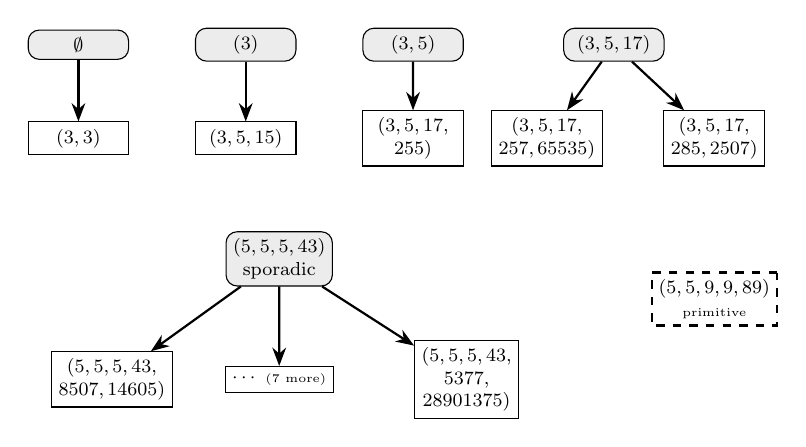
\begin{tikzpicture}[
  seed/.style={draw, rounded corners, fill=gray!15, minimum width=1.5cm,
    font=\footnotesize, align=center, inner sep=3pt},
  lehmer/.style={draw, fill=white, minimum width=1.5cm, font=\footnotesize,
    align=center, inner sep=3pt},
  arr/.style={-{Stealth}, thick},
  scale=0.85, transform shape
]
\node[seed] (s0) at (0,0) {$\emptyset$};
\node[lehmer] (l1) at (0,-1.4) {$(3,3)$};
\node[seed] (s1) at (2.5,0) {$(3)$};
\node[lehmer] (l2) at (2.5,-1.4) {$(3,5,15)$};
\node[seed] (s2) at (5,0) {$(3,5)$};
\node[lehmer] (l3) at (5,-1.4) {$(3,5,17,$\\$255)$};
\node[seed] (s3) at (8,0) {$(3,5,17)$};
\node[lehmer] (l4a) at (7,-1.4) {$(3,5,17,$\\$257,65535)$};
\node[lehmer] (l4b) at (9.5,-1.4) {$(3,5,17,$\\$285,2507)$};

\draw[arr] (s0) -- (l1);
\draw[arr] (s1) -- (l2);
\draw[arr] (s2) -- (l3);
\draw[arr] (s3) -- (l4a);
\draw[arr] (s3) -- (l4b);

\node[seed] (sp1) at (3,-3.2) {$(5,5,5,43)$\\sporadic};
\node[lehmer] (sp1a) at (0.5,-5) {$(5,5,5,43,$\\$8507,14605)$};
\node[lehmer] (sp1b) at (3,-5) {$\cdots$ {\tiny(7 more)}};
\node[lehmer] (sp1c) at (5.8,-5) {$(5,5,5,43,$\\$5377,$\\$28901375)$};
\draw[arr] (sp1) -- (sp1a);
\draw[arr] (sp1) -- (sp1b);
\draw[arr] (sp1) -- (sp1c);

\node[lehmer, dashed, thick] (prim) at (9.5,-3.8) {$(5,5,9,9,89)$\\
  {\tiny primitive}};
\end{tikzpicture}
\caption{A fragment of~$\mathcal{G}_2$.  Rounded: plus-seeds.
Solid: derived Lehmer factorizations.  Dashed: primitive.  The
$(5,5,5,43)$ subtree exhibits both children: the Lehmer descendant
$(5,5,5,43,5375)$ via $x = E$, and the chain extension
$(5,5,5,43,5377)$ via $x = E + 2$.}\label{fig:tree}
\end{figure}


%=====================================================================
\section{Open questions}
%=====================================================================

\begin{enumerate}[label=\arabic*.]
  \item \textbf{Finiteness of primitives.}  All nine known primitive
    $2$-Lehmer factorizations have $|G| \ge 5$.  Are there finitely many
    for each~$k$?

  \item \textbf{Realizability.}  Which spoof factorizations correspond
    to actual integers $n = p_1^{\alpha_1} \cdots p_r^{\alpha_r}$ with
    each $x_i = p_i^{\alpha_i}$ a prime power?

  \item \textbf{Sporadic seed structure.}  Is there a generating mechanism
    for the sporadic plus-seeds, or a secondary recursive structure
    explaining their proliferation?

  \item \textbf{Density of primitives.}  Among our~$39$ factorizations,
    $9$~are primitive (${\approx}23\%$).  Does this proportion converge?
\end{enumerate}


\begin{thebibliography}{9}

\bibitem{H26}
E.~Hasanalizade, \emph{Some remarks on a paper of Molnar and Singh},
Integers \textbf{26} (2026).

\bibitem{L32}
D.~H.~Lehmer, \emph{On Euler's totient function}, Bull.\ Amer.\ Math.\
Soc.\ \textbf{38} (1932), 745--751.

\bibitem{Mfinish}
G.~Molnar, \emph{Closed-form finishing for spoof Lehmer enumeration,
with a complete census at $r \le 7$}, in preparation (2026).

\bibitem{MS26}
G.~Molnar and G.~Singh, \emph{Spoof Lehmer factorizations}, Integers
\textbf{26} (2026), \#A33.

\bibitem{N15}
P.~Nielsen, \emph{Odd perfect numbers, Diophantine equations, and upper
bounds}, Math.\ Comp.\ \textbf{84} (2015), 2549--2567.

\end{thebibliography}

\end{document}
